\section{Corrections and Systematic Uncertainties}
\label{sec:systematics}

The predictions for the signal and background are subject
to the choices made in building the model described thus
far in \sec\ref{sec:www}. If we are to believe our predictions
we must understand how sensitive the predictions are to these choices.
To that end, we also compute the prediction for numerous variations
on the nominal prediction. 
Each one of these variations is called a systematic uncertainty. 
Each systematic uncertainty is designed to assess the sensitivity
to a given choice made when building the model. 
This analysis has almost 50 different systematic
uncertainties, each of which is varied independently. The size of 
each systematic uncertainty
is treated as a separate nuisance parameter
as input to the statistical model used in the interpretation of the model
when compared to data, described later in \sec\ref{sec:measurement}.

The systematic uncertainties can be split up into four categories:
theoretical, methodological, experimental, and luminosity. 
I will summarize them below, in each case giving the 
size of the uncertainties in the three signal regions. 
Some of these variations have 
been mentioned already in previous sections but will be
referred to here again for completeness.

\subsection{Theoretical}
Theoretical uncertainties are those on the signal PDF and 
on the background cross-section predictions.
The motivation for the PDF uncertainties has been described
already in \sec\ref{sec:pdf}. 
There are several uncertainties evaluated on the signal PDF, all of which
are described in more detail in \sec\ref{sec:signal}. These
are the PDF choice, including uncertainties reported by the individual
PDFs, as well as variations in the renormalization and factorization scales.
The effect on the signal prediction from these is around 2-3\%.


The most important MC backgrounds have uncertainties evaluated on their
cross-section.  In particular, these are the uncertainties on the 
normaization of the $WZ$, $ZZ$, $Z\gamma$, $VVV$, $\ttV$, 
and DPS background predictions
described in \sec\ref{sec:bg_estimates} and summarized in \tab\ref{tab:mcnorm}.
Their impact when propogated to the final background prediction
varies by channel. In general, the uncertainty on the $WZ$ prediction is the 
largest, contributing about 2.6\% in the 0 SFOS region around around 8-9\%
in the 1 and 2 SFOS regions.  In the 0 SFOS region, the uncertainty 
on the $VVV$ prediction contributes about 1.4\% and that on the $ZZ$ prediction
is about 0.4\%; all others fall below that. 
In the 1 and 2 SFOS regions the $ZZ$ uncertainty is around 0.6-0.7\%; the
rest are negligible. 


The detailed theoretical uncertainties are summarized for each signal 
region in tab ...... Three tables? Consolidated?


\subsection{Methodological}
The methodological uncertainties are those due to the data-driven
modelling of the fake and charge mis-identification backgrounds,
described in \sec\ref{sec:bg_fake} and \sec\ref{sec:charge_misid},
respectively.
The uncertainty on the fake background is the most important
systematic uncertainty in the analysis, contributing about 60\%
on the final background prediction in the 0 SFOS signal region.
The smaller conribution of the fake background in the 1 and 2 SFOS
regions reduces it in those regions to 5-10\%.
The uncertainty on the charge mis-identification only impacts the 
background prediction in the 0 SFOS channel.  The small size
of this background after the final selection means it only contributes
about 0.5\% to the uncertainty on the final background prediction in that
region.

The detailed methodological uncertainties are summarized for each signal 
region in tab ...... Three tables? Consolidated?

\subsection{Experimental}
The experimental uncertainties are those on the event and object
reconstruction for MC predictions.  That includes both the signal
and background predictions from MC.
Most of the systematic uncertainties evaluated fall in this category.
There are systematic uncertainties taking into account variations
on the identification and reconstruction
efficiency of electrons and muons; and 
the momemtum/energy resolution and scale of reconstructed electrons, muons,
jets, and \MET. In addition, there are uncertainties on the trigger
efficiencies evaluated in MC, effects of pileup, and jet specific uncertainties
like those related to \bee-tagging.

The efficiencies for reconstructing and identifying electrons and muons
are modeled in MC using simulations of the detector. Differences
between the observed efficiencies in data and MC are corrected by scaling
the efficiency in MC, applied using event-by-event weights. 
Uncertainties on these ``scale factors'' are propagated to the event-by-event
weights.  The impact on the final prediction ends up being relatively
small, with sub-percent level contributions coming from both the electron
and muon efficiencies for both the signal and background in all channels.

The momentum and energy measurements for electrons, muons, jets and \MET
must be assessed for their accuracy and precision, usually referred to
as scale and resolution, respectively. The scale of the momentum and energy 
for each object is calibrated using the data and corrected if necessary.
Uncertainties on these calibrations are propogated separately to each object.
The corrections and uncertainties on the scale
from the electrons, muons, and jets propogate to the \MET and a separate
correction and uncertainty on additional contributions to the \MET
not associate with these physics objects (so-called ``soft terms'')
are aslo evaluated. 
The momentum and energy resolution has also been evaluated using the data
for electrons, muons, jets and \MET soft-terms.  Uncertainties due to the
resolution are evaluated by randomly varying the momentum and energy measurements
using a probability distrubtion whose width is determined by the resolution
and centered about the calibrated value. These uncertainties on the scale
and resolution propogate to the final estimate by so-called ``bin migration'',
whereby the uncertainties on the momentum and energy measurement 
for a given object might move it across the threshold for some 
selection cut\footnote{For example, a muon with $\pt = 22 \GeV$ might
be modified during the systematic uncertainty valuation to have instead
$\pt = 19 \GeV$. Thus, with a cut of $\pt > 20 \GeV$, the muon would pass the
cut in the original case but not after variation.}. This can 
then change the overall event selection efficiency. The size of the uncertainties
on the signal and background predictions tend to be around 1-2\% for
all objects and channels.


The efficiency for the events to pass the trigger is evaluated for both 
data and MC.  The efficiencies in MC are corrected to match the data
and an uncertainty is associated with this correction.  They are applied
depending on the trigger that was fired and the objects in the event.
The variations from the uncertainties
modify the event weights which ultimately has an impact on the final predictions.
The uncertainty on the signal and background predictions from the trigger
efficiency end up being only about 0.05-0.07\%  for each channel.

The MC is corrected on an event-by-event basis to match the 
pileup distribution observed in data. This correction depends on the 
MC process. Uncertainties on this correction are varied which again
results in a change in the event-by-event weight for the predictions. The
size of this uncertainty is around 1\% for signal and backgroun in all channels.


Jet specific uncertainties come from variations on the \bee-jet tagging
and \bee-jet mis-identification as well as uncertainties on the jet-vertex
fraction calculations, both described in \sec\ref{sec:object_selection}. They
are also uncertainties related to the construction of jets due to pileup
and the flavor compostion of the jets. These result in modifications
to the observed jet multiplicity leading to bin-migration effects 
for the \bee-veto and jet multiplicity cuts when going to the signal regions.
The resulting uncertainties are...

The detailed experimental uncertainties are summarized for each signal 
region in tab ...... Three tables? Consolidated?

\subsection{Luminosity}
The luminosity delivered by the LHC must be measured in order to determine
how to scale the MC cross-section
predictions to extract the number of events as in \eqn\eqref{eq:lhc_nevents}.
This was described in \sec\ref{sec:subsection_data}. The resuling
uncertainty on the integrated luminosity scales the overall predictions
for the MC signal and background predictions. Thus, the uncertainty 
on the signal prediction in each channel is simply 1.9\%, while the uncertainty
on the background predictions is less since, at around ...,
since it is not estimate purely from MC.



\begin{table}[ht]
\begin{adjustwidth}{-2cm}{-2cm}
\small
\renewcommand{\tabcolsep}{1pt}
\begin{tabular}{|cl||ccccccc|c||c|}
%\begin{tabular}{|cl||p{2.2cm}cccccc|c||c|}
\hline
 & & \multicolumn{8}{c||}{Background} & \\ 
 & & $WZ$ & ZZ & $WWZ$ & $t\overline{t}+V$ & DPI & $Z\gamma$ & Fake & Total & Signal\\ 
 & & &  & $+WZZ$ &  &  &  & (Data) & BG & \\ 
\hline\hline
\multirow{9}{*}{Electron}
&Energy Scale - Low $P_{T}$ & --- &  $^{+0.16}_{+0.00}$  & --- & --- & --- & --- & --- & --- & ---\\ 
\cline{2-11}
&Energy Scale - Material &  $^{+0.39}_{-0.47}$  &  $^{+0.70}_{+0.20}$  &  $^{-0.78}_{+0.80}$  &  $^{-1.41}_{+0.00}$  & --- & --- & --- &  $^{+0.06}_{-0.08}$  &  $^{+0.17}_{-0.05}$ \\ 
\cline{2-11}
&Energy Scale - Presampler &  $^{-0.13}_{+0.14}$  & --- &  $^{-0.00}_{-0.76}$  & --- & --- & --- & --- & --- &  $^{-0.01}_{+0.15}$ \\ 
\cline{2-11}
&Energy Scale - Z$\rightarrow$ ee Gen. & --- & --- & --- & --- & --- & --- & --- & --- & ---\\ 
\cline{2-11}
&Energy Scale - Z$\rightarrow$ ee Meth. &  $^{-0.82}_{+0.65}$  &  $^{-0.12}_{+1.46}$  &  $^{-0.78}_{+1.36}$  &  $^{-1.42}_{-0.02}$  & --- & --- & --- &  $^{-0.28}_{+0.28}$  &  $^{-0.24}_{+0.45}$ \\ 
\cline{2-11}
&Energy Scale - Z$\rightarrow$ ee Stat. &  $^{-0.09}_{+0.07}$  &  $^{+0.14}_{+0.15}$  & --- & --- & --- & --- & --- & --- &  $^{-0.00}_{+0.09}$ \\ 
\cline{2-11}
&Energy Resolution &  $^{+0.02}_{-0.18}$  &  $^{+0.14}_{+0.88}$  &  $^{-1.83}_{+0.06}$  &  $^{-1.23}_{-0.01}$  & --- & --- & --- &  $^{-0.10}_{-0.02}$  &  $^{+0.23}_{+0.05}$ \\ 
\cline{2-11}
&Identification Efficiency &  $^{-1.72}_{+1.73}$  &  $^{-1.74}_{+1.75}$  &  $^{-1.43}_{+1.43}$  &  $^{-1.33}_{+1.34}$  & --- & --- & --- &  $^{-0.59}_{+0.59}$  &  $^{-1.37}_{+1.38}$ \\ 
\cline{2-11}
&Reconstruction Efficiency &  $^{-0.51}_{+0.51}$  &  $^{-0.53}_{+0.53}$  &  $^{-0.52}_{+0.52}$  &  $^{-0.46}_{+0.46}$  & --- & --- & --- &  $^{-0.18}_{+0.18}$  &  $^{-0.45}_{+0.45}$ \\ 
\hline
\multirow{4}{*}{Muon}
&Efficiency &  $^{-0.52}_{+0.52}$  &  $^{-0.53}_{+0.53}$  &  $^{-0.54}_{+0.54}$  &  $^{-0.55}_{+0.55}$  & --- & --- & --- &  $^{-0.19}_{+0.19}$  &  $^{-0.54}_{+0.54}$ \\ 
\cline{2-11}
&Momentum Resolution - ID & --- &  $^{+0.04}_{+0.45}$  &  $^{-0.75}_{-0.00}$  & --- & --- & --- & --- & --- & ---\\ 
\cline{2-11}
&Momentum Resolution - MS & --- &  $^{+0.17}_{-0.15}$  & --- & --- & --- & --- & --- & --- &  $^{+0.00}_{+0.10}$ \\ 
\cline{2-11}
&Momentum Scale &  $^{-0.12}_{+0.12}$  &  $^{-0.01}_{+0.30}$  & --- & --- & --- & --- & --- & --- & ---\\ 
\hline
\multirow{22}{*}{Jet}
&b-tag SF & --- & --- & --- &  $^{-4.22}_{+4.22}$  & --- & --- & --- &  $^{-0.07}_{+0.07}$  & ---\\ 
\cline{2-11}
&c-tag, t-tag SF &  $^{-0.07}_{+0.07}$  &  $^{-0.24}_{+0.24}$  &  $^{-0.32}_{+0.33}$  &  $^{-0.21}_{+0.21}$  & --- & --- & --- & --- & ---\\ 
\cline{2-11}
&mis-tag SF &  $^{-0.25}_{+0.25}$  &  $^{-0.34}_{+0.34}$  &  $^{-0.36}_{+0.36}$  &  $^{-0.41}_{+0.41}$  & --- & --- & --- &  $^{-0.10}_{+0.10}$  &  $^{-0.27}_{+0.27}$ \\ 
\cline{2-11}
&Energy Scale - NP 1 &  $^{+0.55}_{-0.51}$  &  $^{+0.43}_{-0.99}$  &  $^{+2.17}_{-0.77}$  &  $^{+1.53}_{-3.82}$  & --- & --- & --- &  $^{+0.28}_{-0.26}$  &  $^{+0.58}_{-0.46}$ \\ 
\cline{2-11}
&Energy Scale - NP 2 &  $^{-0.98}_{+0.90}$  &  $^{-1.64}_{+1.01}$  &  $^{-0.77}_{+2.17}$  &  $^{-7.20}_{+2.80}$  & --- & --- & --- &  $^{-0.46}_{+0.41}$  &  $^{-0.82}_{+0.85}$ \\ 
\cline{2-11}
&Energy Scale - NP 3 &  $^{+0.42}_{-0.30}$  &  $^{+0.20}_{-0.68}$  &  $^{+2.17}_{-0.77}$  &  $^{+1.53}_{-3.34}$  & --- & --- & --- &  $^{+0.25}_{-0.19}$  &  $^{+0.39}_{-0.33}$ \\ 
\cline{2-11}
&Energy Scale - NP 4 &  $^{-0.10}_{+0.13}$  &  $^{-0.18}_{+0.03}$  &  $^{+0.00}_{+0.51}$  & --- & --- & --- & --- &  $^{-0.03}_{+0.06}$  &  $^{-0.11}_{+0.18}$ \\ 
\cline{2-11}
&Energy Scale - NP 5 &  $^{+0.12}_{-0.09}$  &  $^{+0.03}_{-0.45}$  &  $^{+1.29}_{+0.00}$  & --- & --- & --- & --- &  $^{+0.09}_{-0.04}$  &  $^{+0.17}_{-0.17}$ \\ 
\cline{2-11}
&Energy Scale - NP 6 &  $^{+0.08}_{-0.08}$  & --- & --- & --- & --- & --- & --- & --- &  $^{+0.06}_{-0.09}$ \\ 
\cline{2-11}
&Energy Scale - $\eta$ Model &  $^{+0.89}_{-0.96}$  &  $^{+0.74}_{-1.40}$  &  $^{+3.39}_{-0.77}$  &  $^{+4.18}_{-5.41}$  & --- & --- & --- &  $^{+0.49}_{-0.42}$  &  $^{+0.84}_{-0.86}$ \\ 
\cline{2-11}
&Energy Scale - Stat/Method &  $^{+0.29}_{-0.20}$  &  $^{+0.05}_{-0.64}$  &  $^{+2.13}_{-0.77}$  &  $^{+0.00}_{-1.19}$  & --- & --- & --- &  $^{+0.18}_{-0.13}$  &  $^{+0.31}_{-0.26}$ \\ 
\cline{2-11}
&Energy Scale - Closure & --- & --- & --- & --- & --- & --- & --- & --- & ---\\ 
\cline{2-11}
&Energy Scale - High $P_{T}$ & --- & --- & --- & --- & --- & --- & --- & --- & ---\\ 
\cline{2-11}
&Energy Resolution &  $^{-0.57}_{+0.57}$  &  $^{-0.84}_{+0.84}$  &  $^{-1.55}_{+1.55}$  &  $^{-6.20}_{+6.20}$  & --- & --- & --- &  $^{-0.35}_{+0.35}$  &  $^{-1.06}_{+1.06}$ \\ 
\cline{2-11}
&b-tag JES & --- & --- & --- &  $^{+2.80}_{-5.89}$  & --- & --- & --- &  $^{+0.05}_{-0.10}$  & ---\\ 
\cline{2-11}
&Flavor Composition &  $^{+1.18}_{-1.25}$  &  $^{+1.61}_{-1.83}$  &  $^{+2.17}_{-1.52}$  &  $^{+1.28}_{-3.42}$  & --- & --- & --- &  $^{+0.48}_{-0.51}$  &  $^{+1.15}_{-1.15}$ \\ 
\cline{2-11}
&Flavor Response &  $^{+0.69}_{-0.72}$  &  $^{+0.72}_{-1.31}$  &  $^{+2.17}_{-0.77}$  &  $^{-0.00}_{-0.97}$  & --- & --- & --- &  $^{+0.31}_{-0.28}$  &  $^{+0.73}_{-0.67}$ \\ 
\cline{2-11}
&Pileup - $\mu$ &  $^{+0.12}_{-0.13}$  &  $^{-0.10}_{-0.01}$  &  $^{+1.33}_{+0.00}$  &  $^{+1.27}_{-1.19}$  & --- & --- & --- &  $^{+0.11}_{-0.05}$  &  $^{+0.10}_{-0.09}$ \\ 
\cline{2-11}
&Pileup - \# Primary Vertices &  $^{+0.30}_{-0.33}$  &  $^{-0.07}_{-0.23}$  &  $^{+1.21}_{-0.75}$  &  $^{+1.42}_{-1.24}$  & --- & --- & --- &  $^{+0.16}_{-0.15}$  &  $^{+0.22}_{-0.13}$ \\ 
\cline{2-11}
&Pileup -  $P_{T}$ & --- &  $^{+0.16}_{+0.00}$  & --- & --- & --- & --- & --- & --- & ---\\ 
\cline{2-11}
&Pileup - $\rho$ Topology &  $^{+0.66}_{-0.61}$  &  $^{+0.45}_{-1.15}$  &  $^{+2.17}_{-0.77}$  &  $^{+2.79}_{-5.10}$  & --- & --- & --- &  $^{+0.34}_{-0.31}$  &  $^{+0.61}_{-0.52}$ \\ 
\cline{2-11}
&Vertex Fraction &  $^{-0.08}_{+0.07}$  &  $^{-0.05}_{+0.06}$  & --- &  $^{+0.00}_{+2.27}$  & --- & --- & --- &  $^{-0.02}_{+0.06}$  &  $^{-0.10}_{+0.12}$ \\ 
\hline
\multirow{2}{*}{MET}
&Soft Terms - Resolution &  $^{-0.00}_{-0.23}$  &  $^{+0.18}_{-0.77}$  &  $^{+2.42}_{-2.05}$  &  $^{-2.21}_{+1.30}$  & --- & --- & --- &  $^{+0.08}_{-0.16}$  &  $^{-0.13}_{+0.03}$ \\ 
\cline{2-11}
&Soft Terms - Scale &  $^{+2.46}_{-2.54}$  &  $^{+2.74}_{-1.89}$  &  $^{+1.33}_{-0.25}$  &  $^{+0.00}_{+1.30}$  & --- & --- & --- &  $^{+0.79}_{-0.71}$  &  $^{+1.38}_{-1.74}$ \\ 
\hline
\multirow{2}{*}{Trigger}
&Electron Scale Factor &  $^{-0.09}_{+0.09}$  &  $^{-0.10}_{+0.10}$  & --- & --- & --- & --- & --- & --- &  $^{-0.06}_{+0.06}$ \\ 
\cline{2-11}
&Muon Scale Factor &  $^{-0.18}_{+0.18}$  &  $^{-0.17}_{+0.17}$  & --- & --- & --- & --- & --- &  $^{-0.05}_{+0.05}$  &  $^{-0.07}_{+0.07}$ \\ 
\hline
\multirow{2}{*}{Matrix}
&Electron & --- & --- & --- & --- & --- & --- &  $^{-9.62}_{+9.62}$  &  $^{-6.20}_{+6.20}$  & ---\\ 
\cline{2-11}
\multirow{2}{*}{Method}
&Muon & --- & --- & --- & --- & --- & --- &  $^{-5.06}_{+5.06}$  &  $^{-3.26}_{+3.26}$  & ---\\ 
\cline{2-11}
&b-jet selection & --- & --- & --- & --- & --- & --- &  $^{-83.03}_{+90.19}$  &  $^{-53.52}_{+58.14}$  & ---\\ 
\hline
\multirow{2}{*}{Signal}
&PDF & --- & --- & --- & --- & --- & --- & --- & --- &  $^{+1.70}_{-2.80}$ \\ 
\cline{2-11}
&$\mu_{R}$ and $\mu_{F}$ Choice & --- & --- & --- & --- & --- & --- & --- & --- &  $^{+2.60}_{-2.60}$ \\ 
\hline
\multirow{5}{*}{Normalization}
&WZ &  $^{+10.00}_{-10.00}$  & --- & --- & --- & --- & --- & --- &  $^{+2.63}_{-2.63}$  & ---\\ 
\cline{2-11}
&ZZ & --- &  $^{+15.00}_{-15.00}$  & --- & --- & --- & --- & --- &  $^{+0.42}_{-0.42}$  & ---\\ 
\cline{2-11}
&$WWZ+WZZ$ & --- & --- &  $^{+30.00}_{-30.00}$  & --- & --- & --- & --- &  $^{+1.44}_{-1.44}$  & ---\\ 
\cline{2-11}
&$t\overline{t}+V$ & --- & --- & --- &  $^{+30.00}_{-30.00}$  & --- & --- & --- &  $^{+0.50}_{-0.50}$  & ---\\ 
\cline{2-11}
&DPS & --- & --- & --- & --- &  $^{+50.00}_{-50.00}$  & --- & --- & --- & ---\\ 
\hline
\multirow{1}{*}{Pileup}
&Pileup &  $^{+1.42}_{-1.39}$  &  $^{-0.31}_{-0.12}$  &  $^{+4.11}_{-0.39}$  &  $^{-2.51}_{-1.73}$  & --- & --- & --- &  $^{+0.52}_{-0.42}$  &  $^{+0.92}_{-0.77}$ \\ 
\hline
&Charge Mis-ID &  $^{-1.56}_{+1.58}$  &  $^{-1.23}_{+1.31}$  & --- & --- & --- & --- & --- &  $^{-0.44}_{+0.45}$  & ---\\ 
\hline
&Luminosity &  $^{+2.80}_{-2.80}$  &  $^{+2.80}_{-2.80}$  &  $^{+2.80}_{-2.80}$  &  $^{+2.80}_{-2.80}$  &  $^{+2.80}_{-2.80}$  &  $^{+2.80}_{-2.80}$  &  $^{+2.80}_{-2.80}$  &  $^{+2.80}_{-2.80}$  &  $^{+2.80}_{-2.80}$ \\ 
\hline
&Statistical &  $^{+0.69}_{-0.69}$  &  $^{+5.90}_{-5.90}$  &  $^{+8.83}_{-8.83}$  &  $^{+11.06}_{-11.06}$  & --- & --- &  $^{+17.04}_{-17.04}$  &  $^{+10.99}_{-10.99}$  &  $^{+1.14}_{-1.14}$ \\ 
\hline
\hline
&Yield $\pm$ Sys. $\bigoplus$ Stat. [\%] &  $0.62^{+11.32}_{-11.36}$  &  $0.07^{+17.04}_{-17.06}$  &  $0.11^{+32.67}_{-31.75}$  &  $0.04^{+33.89}_{-36.44}$  &  $<0.01$  &  $<0.01$  &  $1.51^{+92.47}_{-85.50}$  &  $2.35^{+59.75}_{-55.27}$  &  $1.32^{+5.46}_{-5.91}$ \\ 
\hline
\end{tabular}

\caption{All systematic uncertainties in the 0 SFOS signal region.
Uncertainties are shown in percent where the superscript (subscript) in each cell corresponds to the upper (lower) fluctuation
of the given systematic.  Systematics are only shown if the contribution is at least 0.05\% in both directions.}
\label{tab:sys_all_0sfos}
\end{adjustwidth}
\end{table}

\begin{table}[ht]
\begin{adjustwidth}{-2cm}{-2cm}
\small\renewcommand{\tabcolsep}{1pt}
\begin{tabular}{|cl||ccccccc|c||c|}
\hline
 & & \multicolumn{8}{c||}{Background} & \\ 
 & & $WZ$ & ZZ & $WWZ$ & $t\overline{t}+V$ & DPI & $Z\gamma$ & Fake & Total & Signal\\ 
 & & &  & $+WZZ$ &  &  &  & (Data) & BG & \\ 
\hline\hline
\multirow{9}{*}{Electron}
&Energy Scale - Low $P_{T}$ & --- &  $^{+0.09}_{+0.03}$  & --- & --- & --- & --- & --- & --- & ---\\ 
\cline{2-11}
&Energy Scale - Material &  $^{+0.25}_{-0.04}$  &  $^{-0.23}_{+0.07}$  & --- & --- & --- &  $^{-0.00}_{+43.66}$  & --- &  $^{+0.19}_{+0.57}$  &  $^{-0.06}_{+0.04}$ \\ 
\cline{2-11}
&Energy Scale - Presampler & --- &  $^{+0.06}_{+0.06}$  & --- & --- & --- & --- & --- & --- &  $^{+0.02}_{-0.09}$ \\ 
\cline{2-11}
&Energy Scale - Z$\rightarrow$ ee Gen. & --- & --- & --- & --- & --- & --- & --- & --- & ---\\ 
\cline{2-11}
&Energy Scale - Z$\rightarrow$ ee Meth. &  $^{+0.99}_{-0.57}$  &  $^{+1.22}_{-1.17}$  &  $^{+1.01}_{+0.73}$  & --- & --- &  $^{+43.66}_{-0.00}$  & --- &  $^{+1.46}_{-0.49}$  &  $^{+0.57}_{-0.41}$ \\ 
\cline{2-11}
&Energy Scale - Z$\rightarrow$ ee Stat. &  $^{+0.13}_{-0.09}$  &  $^{+0.19}_{-0.00}$  & --- & --- & --- &  $^{+43.66}_{-0.00}$  & --- &  $^{+0.71}_{-0.07}$  &  $^{+0.09}_{-0.11}$ \\ 
\cline{2-11}
&Energy Resolution &  $^{+0.21}_{+0.08}$  &  $^{+0.84}_{-0.50}$  &  $^{-0.00}_{+1.29}$  &  $^{-1.01}_{+0.01}$  & --- &  $^{-0.00}_{+43.66}$  & --- &  $^{+0.20}_{+0.66}$  &  $^{+0.07}_{-0.05}$ \\ 
\cline{2-11}
&Identification Efficiency &  $^{+1.51}_{-1.50}$  &  $^{+1.87}_{-1.85}$  &  $^{+1.42}_{-1.41}$  &  $^{+1.44}_{-1.43}$  &  $^{+0.63}_{-0.62}$  &  $^{+2.02}_{-2.02}$  & --- &  $^{+1.34}_{-1.33}$  &  $^{+1.48}_{-1.47}$ \\ 
\cline{2-11}
&Reconstruction Efficiency &  $^{+0.50}_{-0.50}$  &  $^{+0.59}_{-0.58}$  &  $^{+0.51}_{-0.51}$  &  $^{+0.48}_{-0.48}$  &  $^{+0.29}_{-0.29}$  &  $^{+0.59}_{-0.59}$  & --- &  $^{+0.44}_{-0.44}$  &  $^{+0.49}_{-0.49}$ \\ 
\hline
\multirow{4}{*}{Muon}
&Efficiency &  $^{+0.54}_{-0.54}$  &  $^{+0.50}_{-0.50}$  &  $^{+0.52}_{-0.52}$  &  $^{+0.55}_{-0.55}$  &  $^{+0.32}_{-0.32}$  &  $^{+0.87}_{-0.86}$  & --- &  $^{+0.47}_{-0.47}$  &  $^{+0.53}_{-0.53}$ \\ 
\cline{2-11}
&Momentum Resolution - ID &  $^{+0.20}_{-0.05}$  &  $^{+0.13}_{-0.16}$  & --- &  $^{+0.00}_{-0.63}$  & --- &  $^{+42.28}_{-0.00}$  & --- &  $^{+0.74}_{-0.05}$  & ---\\ 
\cline{2-11}
&Momentum Resolution - MS &  $^{+0.55}_{+0.11}$  &  $^{+0.84}_{+0.06}$  &  $^{+0.22}_{-0.00}$  &  $^{+0.57}_{+0.00}$  & --- &  $^{+9.96}_{-0.00}$  & --- &  $^{+0.61}_{+0.09}$  &  $^{+0.07}_{+0.04}$ \\ 
\cline{2-11}
&Momentum Scale &  $^{+0.21}_{-0.07}$  & --- & --- & --- & --- & --- & --- &  $^{+0.17}_{-0.06}$  &  $^{+0.05}_{-0.10}$ \\ 
\hline
\multirow{22}{*}{Jet}
&b-tag SF & --- & --- & --- &  $^{+4.94}_{-4.94}$  & --- & --- & --- & --- & ---\\ 
\cline{2-11}
&c-tag, t-tag SF &  $^{+0.05}_{-0.05}$  &  $^{+0.72}_{-0.72}$  &  $^{+0.48}_{-0.48}$  &  $^{+0.20}_{-0.20}$  & --- & --- & --- &  $^{+0.07}_{-0.07}$  & ---\\ 
\cline{2-11}
&mis-tag SF &  $^{+0.34}_{-0.34}$  &  $^{+0.38}_{-0.38}$  &  $^{+0.60}_{-0.60}$  &  $^{+0.48}_{-0.48}$  &  $^{+1.23}_{-1.23}$  &  $^{+0.61}_{-0.61}$  & --- &  $^{+0.30}_{-0.30}$  &  $^{+0.30}_{-0.30}$ \\ 
\cline{2-11}
&Energy Scale - NP 1 &  $^{-0.64}_{+0.89}$  &  $^{-0.83}_{+1.77}$  &  $^{-0.58}_{+1.68}$  &  $^{-3.25}_{+1.19}$  & --- & --- & --- &  $^{-0.57}_{+0.80}$  &  $^{-0.48}_{+0.39}$ \\ 
\cline{2-11}
&Energy Scale - NP 2 &  $^{+1.29}_{-0.93}$  &  $^{+2.59}_{-1.70}$  &  $^{+1.59}_{-0.59}$  &  $^{+2.93}_{-3.91}$  & --- & --- & --- &  $^{+1.16}_{-0.83}$  &  $^{+0.64}_{-0.80}$ \\ 
\cline{2-11}
&Energy Scale - NP 3 &  $^{-0.39}_{+0.65}$  &  $^{-0.55}_{+1.08}$  &  $^{-0.58}_{+1.67}$  &  $^{-2.81}_{+0.18}$  & --- & --- & --- &  $^{-0.35}_{+0.58}$  &  $^{-0.37}_{+0.30}$ \\ 
\cline{2-11}
&Energy Scale - NP 4 &  $^{+0.20}_{-0.07}$  &  $^{+0.63}_{-0.03}$  &  $^{+0.55}_{+0.00}$  &  $^{-1.01}_{-0.91}$  & --- & --- & --- &  $^{+0.18}_{-0.06}$  &  $^{+0.07}_{-0.11}$ \\ 
\cline{2-11}
&Energy Scale - NP 5 &  $^{-0.08}_{+0.14}$  &  $^{-0.12}_{+0.62}$  &  $^{+0.00}_{+0.55}$  &  $^{-0.91}_{+0.11}$  & --- & --- & --- &  $^{-0.07}_{+0.14}$  &  $^{-0.15}_{+0.08}$ \\ 
\cline{2-11}
&Energy Scale - NP 6 &  $^{-0.08}_{+0.21}$  &  $^{-0.00}_{+0.45}$  &  $^{+0.00}_{+0.55}$  & --- & --- & --- & --- &  $^{-0.06}_{+0.19}$  &  $^{-0.07}_{+0.03}$ \\ 
\cline{2-11}
&Energy Scale - $\eta$ Model &  $^{-0.83}_{+1.23}$  &  $^{-1.89}_{+1.32}$  &  $^{+0.00}_{+1.75}$  &  $^{-2.01}_{+2.31}$  & --- & --- & --- &  $^{-0.75}_{+1.06}$  &  $^{-0.80}_{+0.58}$ \\ 
\cline{2-11}
&Energy Scale - Stat/Method &  $^{-0.23}_{+0.38}$  &  $^{-0.44}_{+0.75}$  &  $^{+0.00}_{+0.55}$  &  $^{-0.91}_{+1.13}$  & --- & --- & --- &  $^{-0.20}_{+0.34}$  &  $^{-0.21}_{+0.12}$ \\ 
\cline{2-11}
&Energy Scale - Closure  & --- & --- & --- & --- & --- & --- & --- & --- & ---\\ 
\cline{2-11}
&Energy Scale - High $P_{T}$ & --- & --- & --- & --- & --- & --- & --- & --- & ---\\ 
\cline{2-11}
&Energy Resolution &  $^{+0.32}_{-0.32}$  &  $^{+2.34}_{-2.34}$  &  $^{+0.43}_{-0.43}$  &  $^{+6.44}_{-6.44}$  &  $^{+0.24}_{-0.24}$  &  $^{+2.63}_{-2.63}$  & --- &  $^{+0.41}_{-0.41}$  &  $^{+1.31}_{-1.31}$ \\ 
\cline{2-11}
&b-tag JES & --- &  $^{-0.09}_{+0.00}$  & --- &  $^{-1.52}_{+1.93}$  & --- & --- & --- & --- & ---\\ 
\cline{2-11}
&Flavor Composition &  $^{-1.27}_{+1.54}$  &  $^{-2.87}_{+2.85}$  &  $^{-0.60}_{+2.01}$  &  $^{-6.35}_{+4.39}$  & --- &  $^{+0.03}_{+2.56}$  & --- &  $^{-1.16}_{+1.42}$  &  $^{-0.99}_{+0.92}$ \\ 
\cline{2-11}
&Flavor Response &  $^{-0.76}_{+0.97}$  &  $^{-1.00}_{+2.12}$  &  $^{-0.59}_{+1.58}$  &  $^{-2.76}_{+1.01}$  & --- & --- & --- &  $^{-0.67}_{+0.88}$  &  $^{-0.67}_{+0.48}$ \\ 
\cline{2-11}
&Pileup - $\mu$ &  $^{-0.21}_{+0.19}$  &  $^{-0.41}_{+1.00}$  &  $^{-0.00}_{+0.81}$  &  $^{-0.90}_{-0.42}$  & --- & --- & --- &  $^{-0.19}_{+0.20}$  &  $^{-0.24}_{+0.18}$ \\ 
\cline{2-11}
&Pileup - \# Primary Vertices &  $^{-0.29}_{+0.34}$  &  $^{-0.39}_{+1.27}$  &  $^{-0.58}_{+1.94}$  &  $^{-4.73}_{+1.86}$  & --- & --- & --- &  $^{-0.27}_{+0.35}$  &  $^{-0.24}_{+0.22}$ \\ 
\cline{2-11}
&Pileup -  $P_{T}$ &  $^{+0.00}_{+0.07}$  &  $^{-0.10}_{-0.13}$  & --- & --- & --- & --- & --- &  $^{-0.00}_{+0.05}$  & ---\\ 
\cline{2-11}
&Pileup - $\rho$ Topology &  $^{-0.51}_{+0.86}$  &  $^{-0.49}_{+1.69}$  &  $^{-0.58}_{+1.95}$  &  $^{-2.85}_{+0.87}$  & --- & --- & --- &  $^{-0.44}_{+0.78}$  &  $^{-0.63}_{+0.49}$ \\ 
\cline{2-11}
&Vertex Fraction &  $^{+0.04}_{-0.12}$  &  $^{+0.30}_{-0.34}$  &  $^{+0.01}_{-0.70}$  &  $^{+1.89}_{-1.66}$  & --- & --- & --- &  $^{+0.05}_{-0.12}$  &  $^{+0.15}_{-0.13}$ \\ 
\hline
\multirow{2}{*}{MET}
&Soft Terms - Resolution &  $^{+0.22}_{+0.32}$  &  $^{-0.05}_{+0.25}$  &  $^{+0.35}_{-1.38}$  &  $^{+0.22}_{-2.13}$  & --- &  $^{-4.60}_{+51.75}$  & --- &  $^{+0.11}_{+0.96}$  &  $^{-0.47}_{-0.24}$ \\ 
\cline{2-11}
&Soft Terms - Scale &  $^{+0.22}_{+0.33}$  &  $^{+5.23}_{-5.90}$  &  $^{-1.57}_{-1.14}$  &  $^{-1.65}_{-1.63}$  & --- &  $^{+44.87}_{-9.73}$  & --- &  $^{+0.98}_{-0.11}$  &  $^{-0.71}_{+0.71}$ \\ 
\hline
\multirow{2}{*}{Trigger}
&Electron Scale Factor &  $^{+0.06}_{-0.06}$  &  $^{+0.10}_{-0.10}$  & --- &  $^{+0.05}_{-0.05}$  & --- & --- & --- &  $^{+0.05}_{-0.05}$  &  $^{+0.05}_{-0.05}$ \\ 
\cline{2-11}
&Muon Scale Factor &  $^{+0.08}_{-0.08}$  &  $^{+0.13}_{-0.13}$  & --- & --- & --- &  $^{+0.26}_{-0.26}$  & --- &  $^{+0.07}_{-0.07}$  &  $^{+0.07}_{-0.07}$ \\ 
\hline
\multirow{2}{*}{Matrix}
&Electron & --- & --- & --- & --- & --- & --- &  $^{+36.50}_{-36.50}$  &  $^{+4.69}_{-4.69}$  & ---\\ 
\cline{2-11}
\multirow{2}{*}{Method}
&Muon & --- & --- & --- & --- & --- & --- &  $^{+5.11}_{-5.11}$  &  $^{+0.66}_{-0.66}$  & ---\\ 
\cline{2-11}
&b-jet selection & --- & --- & --- & --- & --- & --- &  $^{+91.16}_{-83.90}$  &  $^{+11.72}_{-10.79}$  & ---\\ 
\hline
\multirow{2}{*}{Signal}
&PDF & --- & --- & --- & --- & --- & --- & --- & --- &  $^{+1.70}_{-2.80}$ \\ 
\cline{2-11}
&$\mu_{R}$ and $\mu_{F}$ Choice & --- & --- & --- & --- & --- & --- & --- & --- &  $^{+2.60}_{-2.60}$ \\ 
\hline
\multirow{5}{*}{Normalization}
&WZ &  $^{+10.00}_{-10.00}$  & --- & --- & --- & --- & --- & --- &  $^{+8.05}_{-8.05}$  & ---\\ 
\cline{2-11}
&ZZ & --- &  $^{+15.00}_{-15.00}$  & --- & --- & --- & --- & --- &  $^{+0.59}_{-0.59}$  & ---\\ 
\cline{2-11}
&$WWZ+WZZ$ & --- & --- &  $^{+30.00}_{-30.00}$  & --- & --- & --- & --- &  $^{+0.28}_{-0.28}$  & ---\\ 
\cline{2-11}
&$t\overline{t}+V$ & --- & --- & --- &  $^{+30.00}_{-30.00}$  & --- & --- & --- &  $^{+0.10}_{-0.10}$  & ---\\ 
\cline{2-11}
&DPS & --- & --- & --- & --- &  $^{+50.00}_{-50.00}$  & --- & --- & --- & ---\\ 
\hline
\multirow{1}{*}{Pileup}
&Pileup &  $^{+0.02}_{-0.35}$  &  $^{+4.10}_{-4.30}$  &  $^{+0.19}_{+1.80}$  &  $^{+0.02}_{-2.52}$  &  $^{+3.42}_{-28.56}$  &  $^{+1.77}_{+38.30}$  & --- &  $^{+0.20}_{+0.07}$  &  $^{-1.30}_{+1.10}$ \\ 
\hline
&Charge Mis-ID & --- & --- & --- & --- & --- & --- & --- & --- & ---\\ 
\hline
&Luminosity &  $^{+2.80}_{-2.80}$  &  $^{+2.80}_{-2.80}$  &  $^{+2.80}_{-2.80}$  &  $^{+2.80}_{-2.80}$  &  $^{+2.80}_{-2.80}$  &  $^{+2.80}_{-2.80}$  &  $^{+2.80}_{-2.80}$  &  $^{+2.80}_{-2.80}$  &  $^{+2.80}_{-2.80}$ \\ 
\hline
&Statistical &  $^{+1.22}_{-1.22}$  &  $^{+2.75}_{-2.75}$  &  $^{+7.95}_{-7.95}$  &  $^{+9.45}_{-9.45}$  &  $^{+91.36}_{-91.36}$  &  $^{+64.37}_{-64.37}$  &  $^{+18.02}_{-18.02}$  &  $^{+2.67}_{-2.67}$  &  $^{+1.12}_{-1.12}$ \\ 
\hline
\hline
&Yield $\pm$ Sys. $\bigoplus$ Stat. [\%] &  $11.89^{+11.09}_{-10.84}$  &  $0.58^{+18.18}_{-17.98}$  &  $0.14^{+31.75}_{-31.35}$  &  $0.05^{+33.44}_{-34.78}$  &  $0.01^{+104.25}_{-108.04}$  &  $0.20^{+140.86}_{-65.42}$  &  $1.90^{+100.01}_{-93.44}$  &  $14.77^{+16.00}_{-15.02}$  &  $1.39^{+5.27}_{-5.88}$ \\ 
\hline
\end{tabular}

\caption{All systematic uncertainties in the 1 SFOS signal region.
Uncertainties are shown in percent where the superscript (subscript) in each cell corresponds to the upper (lower) fluctuation
of the given systematic. 
Systematics are only shown if the contribution is at least 0.05\% in both directions.  }
\label{tab:sys_all_1sfos}
\end{adjustwidth}
\end{table}

\begin{table}[ht]
\begin{adjustwidth}{-2cm}{-2cm}
\small\renewcommand{\tabcolsep}{1pt}
\begin{tabular}{|cl||ccccccc|c||c|}
\hline
 & & \multicolumn{8}{c||}{Background} & \\ 
 & & $WZ$ & ZZ & $WWZ$ & $t\overline{t}+V$ & DPI & $Z\gamma$ & Fake & Total & Signal\\ 
 & & &  & $+WZZ$ &  &  &  & (Data) & BG & \\ 
\hline\hline
\multirow{9}{*}{Electron}
&Energy Scale - Low $P_{T}$ & --- & --- & --- & --- & --- & --- & --- & --- & ---\\ 
\cline{2-11}
&Energy Scale - Material &  $^{-0.17}_{-0.21}$  &  $^{-0.22}_{-0.13}$  &  $^{+0.23}_{+0.00}$  & --- & --- &  $^{+0.00}_{-0.26}$  & --- &  $^{-0.16}_{-0.19}$  &  $^{+0.00}_{-0.11}$ \\ 
\cline{2-11}
&Energy Scale - Presampler & --- &  $^{+0.10}_{-0.08}$  &  $^{+0.00}_{+0.23}$  & --- & --- & --- & --- & --- & ---\\ 
\cline{2-11}
&Energy Scale - Z$\rightarrow$ ee Gen. & --- & --- & --- & --- & --- & --- & --- & --- & ---\\ 
\cline{2-11}
&Energy Scale - Z$\rightarrow$ ee Meth. &  $^{-0.65}_{+0.44}$  &  $^{-0.45}_{+0.35}$  &  $^{-0.49}_{+0.17}$  &  $^{-2.34}_{-0.00}$  & --- &  $^{-0.26}_{+0.00}$  & --- &  $^{-0.60}_{+0.41}$  &  $^{-0.31}_{+0.21}$ \\ 
\cline{2-11}
&Energy Scale - Z$\rightarrow$ ee Stat. &  $^{-0.11}_{+0.08}$  & --- & --- & --- & --- & --- & --- &  $^{-0.10}_{+0.07}$  &  $^{+0.05}_{+0.05}$ \\ 
\cline{2-11}
&Energy Resolution &  $^{-0.18}_{-0.08}$  &  $^{-0.28}_{-0.10}$  &  $^{+0.15}_{+0.22}$  &  $^{+1.17}_{+0.00}$  & --- &  $^{+0.00}_{-86.94}$  & --- &  $^{-0.16}_{-1.00}$  &  $^{-0.24}_{-0.06}$ \\ 
\cline{2-11}
&Identification Efficiency &  $^{-0.94}_{+0.96}$  &  $^{-0.60}_{+0.61}$  &  $^{-1.18}_{+1.21}$  &  $^{-0.74}_{+0.76}$  &  $^{-1.55}_{+1.58}$  &  $^{-2.70}_{+2.73}$  & --- &  $^{-0.90}_{+0.92}$  &  $^{-0.92}_{+0.94}$ \\ 
\cline{2-11}
&Reconstruction Efficiency &  $^{-0.32}_{+0.32}$  &  $^{-0.20}_{+0.20}$  &  $^{-0.42}_{+0.43}$  &  $^{-0.27}_{+0.28}$  &  $^{-0.49}_{+0.49}$  &  $^{-1.24}_{+1.25}$  & --- &  $^{-0.31}_{+0.31}$  &  $^{-0.31}_{+0.31}$ \\ 
\hline
\multirow{4}{*}{Muon}
&Efficiency &  $^{-0.72}_{+0.73}$  &  $^{-0.85}_{+0.85}$  &  $^{-0.66}_{+0.67}$  &  $^{-0.75}_{+0.75}$  &  $^{-0.47}_{+0.48}$  & --- & --- &  $^{-0.68}_{+0.69}$  &  $^{-0.71}_{+0.71}$ \\ 
\cline{2-11}
&Momentum Resolution - ID &  $^{-0.41}_{+0.07}$  &  $^{-0.28}_{+0.46}$  & --- & --- & --- & --- & --- &  $^{-0.37}_{+0.09}$  &  $^{-0.15}_{+0.15}$ \\ 
\cline{2-11}
&Momentum Resolution - MS &  $^{-0.05}_{+0.41}$  &  $^{-0.06}_{-0.40}$  &  $^{+0.00}_{+1.03}$  & --- & --- & --- & --- &  $^{-0.05}_{+0.35}$  &  $^{-0.07}_{-0.38}$ \\ 
\cline{2-11}
&Momentum Scale &  $^{-0.18}_{+0.25}$  &  $^{-0.26}_{+0.18}$  & --- & --- & --- & --- & --- &  $^{-0.17}_{+0.23}$  &  $^{-0.13}_{+0.12}$ \\ 
\hline
\multirow{22}{*}{Jet}
&b-tag SF & --- & --- & --- &  $^{-4.83}_{+4.83}$  & --- & --- & --- & --- & ---\\ 
\cline{2-11}
&c-tag, t-tag SF &  $^{-0.06}_{+0.06}$  &  $^{-0.64}_{+0.64}$  &  $^{-0.89}_{+0.89}$  &  $^{-0.62}_{+0.62}$  & --- & --- & --- &  $^{-0.09}_{+0.09}$  & ---\\ 
\cline{2-11}
&mis-tag SF &  $^{-0.36}_{+0.36}$  &  $^{-0.34}_{+0.34}$  &  $^{-0.37}_{+0.37}$  &  $^{-0.19}_{+0.19}$  &  $^{-0.49}_{+0.49}$  &  $^{-2.02}_{+2.02}$  & --- &  $^{-0.36}_{+0.36}$  &  $^{-0.30}_{+0.30}$ \\ 
\cline{2-11}
&Energy Scale - NP 1 &  $^{+0.43}_{-0.40}$  &  $^{+0.87}_{-0.97}$  & --- &  $^{+1.93}_{-1.04}$  & --- & --- & --- &  $^{+0.43}_{-0.40}$  &  $^{+0.22}_{-0.46}$ \\ 
\cline{2-11}
&Energy Scale - NP 2 &  $^{-0.91}_{+0.69}$  &  $^{-1.15}_{+1.18}$  &  $^{-2.17}_{+0.01}$  &  $^{-3.09}_{+12.54}$  & --- &  $^{-86.94}_{-0.03}$  & --- &  $^{-1.81}_{+0.69}$  &  $^{-0.87}_{+0.51}$ \\ 
\cline{2-11}
&Energy Scale - NP 3 &  $^{+0.24}_{-0.22}$  &  $^{+0.40}_{-0.59}$  & --- &  $^{+2.06}_{-1.04}$  & --- & --- & --- &  $^{+0.24}_{-0.23}$  &  $^{+0.18}_{-0.34}$ \\ 
\cline{2-11}
&Energy Scale - NP 4 &  $^{-0.06}_{+0.02}$  &  $^{-0.24}_{+0.04}$  & --- &  $^{-0.00}_{+2.06}$  & --- & --- & --- &  $^{-0.07}_{+0.03}$  &  $^{-0.07}_{+0.09}$ \\ 
\cline{2-11}
&Energy Scale - NP 5 &  $^{+0.07}_{-0.03}$  &  $^{-0.17}_{-0.20}$  & --- &  $^{+2.06}_{-0.00}$  & --- & --- & --- &  $^{+0.06}_{-0.04}$  &  $^{+0.16}_{-0.13}$ \\ 
\cline{2-11}
&Energy Scale - NP 6 & --- &  $^{-0.06}_{-0.23}$  & --- &  $^{+2.06}_{-0.00}$  & --- & --- & --- & --- &  $^{+0.07}_{-0.06}$ \\ 
\cline{2-11}
&Energy Scale - $\eta$ Model &  $^{+0.70}_{-0.97}$  &  $^{+0.68}_{-0.52}$  &  $^{+0.80}_{-2.15}$  &  $^{+4.39}_{-0.80}$  & --- &  $^{-0.02}_{-29.59}$  & --- &  $^{+0.66}_{-1.21}$  &  $^{+0.38}_{-0.90}$ \\ 
\cline{2-11}
&Energy Scale - Stat/Method &  $^{+0.16}_{-0.11}$  &  $^{+0.07}_{-0.34}$  & --- &  $^{+2.06}_{-0.00}$  & --- & --- & --- &  $^{+0.15}_{-0.12}$  &  $^{+0.22}_{-0.21}$ \\ 
\cline{2-11}
&Energy Scale - Closure & --- & --- & --- & --- & --- & --- & --- & --- & ---\\ 
\cline{2-11}
&Energy Scale - High $P_{T}$ & --- & --- & --- & --- & --- & --- & --- & --- & ---\\ 
\cline{2-11}
&Energy Resolution &  $^{-1.31}_{+1.31}$  &  $^{-2.13}_{+2.13}$  & --- &  $^{-16.44}_{+16.44}$  &  $^{-42.30}_{+42.30}$  &  $^{-86.96}_{+86.96}$  & --- &  $^{-2.31}_{+2.31}$  &  $^{-0.99}_{+0.99}$ \\ 
\cline{2-11}
&b-tag JES & --- &  $^{+0.12}_{-0.10}$  & --- &  $^{+7.73}_{-0.10}$  & --- & --- & --- & --- & ---\\ 
\cline{2-11}
&Flavor Composition &  $^{+1.18}_{-1.31}$  &  $^{+2.02}_{-1.76}$  &  $^{+0.06}_{-2.17}$  &  $^{+4.82}_{-1.06}$  & --- &  $^{-0.04}_{-86.94}$  & --- &  $^{+1.15}_{-2.19}$  &  $^{+0.73}_{-1.12}$ \\ 
\cline{2-11}
&Flavor Response &  $^{+0.60}_{-0.58}$  &  $^{+0.90}_{-1.20}$  &  $^{+0.01}_{-1.12}$  &  $^{+3.42}_{-1.04}$  & --- &  $^{-0.02}_{-86.94}$  & --- &  $^{+0.58}_{-1.51}$  &  $^{+0.41}_{-0.58}$ \\ 
\cline{2-11}
&Pileup - $\mu$ &  $^{+0.16}_{-0.12}$  & --- & --- & --- & --- & --- & --- &  $^{+0.14}_{-0.11}$  &  $^{+0.05}_{-0.07}$ \\ 
\cline{2-11}
&Pileup - \# Primary Vertices &  $^{+0.29}_{-0.20}$  &  $^{+0.81}_{-0.58}$  & --- &  $^{+2.06}_{-3.23}$  & --- & --- & --- &  $^{+0.30}_{-0.21}$  &  $^{+0.11}_{-0.18}$ \\ 
\cline{2-11}
&Pileup -  $P_{T}$ &  $^{-0.07}_{+0.02}$  &  $^{-0.11}_{-0.09}$  & --- & --- & --- & --- & --- &  $^{-0.06}_{+0.02}$  & ---\\ 
\cline{2-11}
&Pileup - $\rho$ Topology &  $^{+0.35}_{-0.42}$  &  $^{+0.40}_{-0.91}$  &  $^{+0.01}_{-2.14}$  &  $^{+12.68}_{-1.04}$  & --- &  $^{-0.02}_{-86.94}$  & --- &  $^{+0.36}_{-1.36}$  &  $^{+0.26}_{-0.50}$ \\ 
\cline{2-11}
&Vertex Fraction &  $^{-0.10}_{+0.28}$  &  $^{-0.14}_{+0.44}$  & --- &  $^{+0.00}_{+3.47}$  & --- & --- & --- &  $^{-0.10}_{+0.28}$  &  $^{-0.06}_{+0.07}$ \\ 
\hline
\multirow{2}{*}{MET}
&Soft Terms - Resolution & --- &  $^{+1.79}_{+1.21}$  &  $^{-1.32}_{+1.74}$  &  $^{-3.94}_{-4.70}$  &  $^{-55.97}_{-55.97}$  &  $^{+57.36}_{-86.94}$  & --- &  $^{+0.56}_{-1.00}$  &  $^{+0.23}_{-0.26}$ \\ 
\cline{2-11}
&Soft Terms - Scale &  $^{-1.29}_{+1.16}$  &  $^{-5.71}_{+8.67}$  &  $^{+0.92}_{+1.08}$  &  $^{-4.41}_{-1.04}$  &  $^{-55.97}_{+0.00}$  &  $^{-86.94}_{+57.36}$  & --- &  $^{-2.46}_{+2.04}$  &  $^{-0.13}_{-0.20}$ \\ 
\hline
\multirow{2}{*}{Trigger}
&Electron Scale Factor & --- & --- & --- & --- & --- & --- & --- & --- & ---\\ 
\cline{2-11}
&Muon Scale Factor &  $^{-0.22}_{+0.22}$  &  $^{-0.31}_{+0.31}$  &  $^{-0.19}_{+0.19}$  &  $^{-0.24}_{+0.24}$  &  $^{-0.44}_{+0.44}$  & --- & --- &  $^{-0.21}_{+0.21}$  &  $^{-0.20}_{+0.20}$ \\ 
\hline
\multirow{2}{*}{Matrix}
&Electron & --- & --- & --- & --- & --- & --- &  $^{-22.21}_{+22.21}$  &  $^{-1.07}_{+1.07}$  & ---\\ 
\cline{2-11}
\multirow{2}{*}{Method}
&Muon & --- & --- & --- & --- & --- & --- &  $^{-6.80}_{+6.80}$  &  $^{-0.33}_{+0.33}$  & ---\\ 
\cline{2-11}
&b-jet selection & --- & --- & --- & --- & --- & --- &  $^{-84.82}_{+87.19}$  &  $^{-4.08}_{+4.20}$  & ---\\ 
\hline
\multirow{2}{*}{Signal}
&PDF & --- & --- & --- & --- & --- & --- & --- & --- &  $^{+1.70}_{-2.80}$ \\ 
\cline{2-11}
&$\mu_{R}$ and $\mu_{F}$ Choice & --- & --- & --- & --- & --- & --- & --- & --- &  $^{+2.60}_{-2.60}$ \\ 
\hline
\multirow{5}{*}{Normalization}
&WZ &  $^{+10.00}_{-10.00}$  & --- & --- & --- & --- & --- & --- &  $^{+8.83}_{-8.83}$  & ---\\ 
\cline{2-11}
&ZZ & --- &  $^{+15.00}_{-15.00}$  & --- & --- & --- & --- & --- &  $^{+0.70}_{-0.70}$  & ---\\ 
\cline{2-11}
&$WWZ+WZZ$ & --- & --- &  $^{+30.00}_{-30.00}$  & --- & --- & --- & --- &  $^{+0.23}_{-0.23}$  & ---\\ 
\cline{2-11}
&$t\overline{t}+V$ & --- & --- & --- &  $^{+30.00}_{-30.00}$  & --- & --- & --- &  $^{+0.07}_{-0.07}$  & ---\\ 
\cline{2-11}
&DPS & --- & --- & --- & --- &  $^{+50.00}_{-50.00}$  & --- & --- &  $^{+0.11}_{-0.11}$  & ---\\ 
\hline
\multirow{1}{*}{Pileup}
&Pileup &  $^{-1.12}_{+0.92}$  &  $^{-6.32}_{+8.04}$  &  $^{-6.69}_{+5.63}$  &  $^{+0.04}_{+0.19}$  &  $^{+2.25}_{-7.67}$  &  $^{-7.18}_{+16.49}$  & --- &  $^{-1.40}_{+1.39}$  &  $^{+1.50}_{-1.24}$ \\ 
\hline
&Charge Mis-ID & --- & --- & --- & --- & --- & --- & --- & --- & ---\\ 
\hline
&Luminosity &  $^{+2.80}_{-2.80}$  &  $^{+2.80}_{-2.80}$  &  $^{+2.80}_{-2.80}$  &  $^{+2.80}_{-2.80}$  &  $^{+2.80}_{-2.80}$  &  $^{+2.80}_{-2.80}$  &  $^{+2.80}_{-2.80}$  &  $^{+2.80}_{-2.80}$  &  $^{+2.80}_{-2.80}$ \\ 
\hline
&Statistical &  $^{+1.39}_{-1.39}$  &  $^{+2.27}_{-2.27}$  &  $^{+10.19}_{-10.19}$  &  $^{+13.84}_{-13.84}$  &  $^{+70.18}_{-70.18}$  &  $^{+87.92}_{-87.92}$  &  $^{+32.33}_{-32.33}$  &  $^{+2.20}_{-2.20}$  &  $^{+1.70}_{-1.70}$ \\ 
\hline
\hline
&Yield $\pm$ Sys. $\bigoplus$ Stat. [\%] &  $9.05^{+10.92}_{-11.01}$  &  $0.48^{+19.95}_{-18.07}$  &  $0.08^{+32.46}_{-32.88}$  &  $0.02^{+43.23}_{-38.53}$  &  $0.02^{+96.08}_{-136.68}$  &  $0.11^{+148.87}_{-262.96}$  &  $0.49^{+95.89}_{-93.74}$  &  $10.25^{+11.26}_{-11.86}$  &  $0.60^{+5.17}_{-5.81}$ \\ 
\hline
\end{tabular}

\caption{All systematic uncertainties in the 2 SFOS signal region.
Uncertainties are shown in percent where the superscript (subscript) in each cell corresponds to the upper (lower) fluctuation
of the given systematic. 
Systematics are only shown if the contribution is at least 0.05\% in both directions. }
\label{tab:sys_all_2sfos}
\end{adjustwidth}
\end{table}


%\begin{table}[ht]
%\centering
%\renewcommand{\tabcolsep}{2pt}
\small\begin{tabular}{c|rclrclrcl}
\hline
\hline
 & \multicolumn{3}{c}{0 SFOS} & \multicolumn{3}{c}{1 SFOS} & \multicolumn{3}{c}{2 SFOS}\\ 
\hline
$WZ$ &  $0.6176 $&$\pm$&$ 0.0043~^{+0.0699}_{-0.0701}$ &  $11.89 $&$\pm$&$ 0.14~^{+1.32}_{-1.29}$ &  $9.05 $&$\pm$&$ 0.13~^{+0.99}_{-1.00}$\\ 
ZZ &  $0.0658 $&$\pm$&$ 0.0039~^{+0.0112}_{-0.0112}$ &  $0.581 $&$\pm$&$ 0.016~^{+0.106}_{-0.105}$ &  $0.477 $&$\pm$&$ 0.011~^{+0.095}_{-0.086}$\\ 
$WWZ+WZZ$ &  $0.1126 $&$\pm$&$ 0.0099~^{+0.0146}_{-0.0117}$ &  $0.140 $&$\pm$&$ 0.011~^{+0.015}_{-0.013}$ &  $0.0785 $&$\pm$&$ 0.0080~^{+0.0097}_{-0.0106}$\\ 
$t\overline{t}+$V &  $0.0388 $&$\pm$&$ 0.0043~^{+0.0061}_{-0.0077}$ &  $0.0503 $&$\pm$&$ 0.0048~^{+0.0074}_{-0.0089}$ &  $0.0239 $&$\pm$&$ 0.0033~^{+0.0074}_{-0.0058}$\\ 
DPS &  $0.0 $&$\pm$&$ 0.0~^{+0.0}_{-0.0}$ &  $0.0088 $&$\pm$&$ 0.0080~^{+0.0080}_{-0.0084}$ &  $0.023 $&$\pm$&$ 0.016~^{+0.019}_{-0.029}$\\ 
$Z\gamma$ &  $0.0 $&$\pm$&$ 0.0~^{+0.0}_{-0.0}$ &  $0.20 $&$\pm$&$ 0.13~^{+0.29}_{-0.13}$ &  $0.110 $&$\pm$&$ 0.096~^{+0.163}_{-0.288}$\\ 
Fake &  $1.51 $&$\pm$&$ 0.26~^{+1.40}_{-1.29}$ &  $1.90 $&$\pm$&$ 0.34~^{+1.90}_{-1.77}$ &  $0.49 $&$\pm$&$ 0.16~^{+0.47}_{-0.46}$\\ 
Signal &  $1.320 $&$\pm$&$ 0.015~^{+0.072}_{-0.078}$ &  $1.369 $&$\pm$&$ 0.015~^{+0.072}_{-0.080}$ &  $0.603 $&$\pm$&$ 0.010~^{+0.031}_{-0.035}$\\ 
\hline
Total Background &  $2.35 $&$\pm$&$ 0.26~^{+1.40}_{-1.30}$ &  $14.77 $&$\pm$&$ 0.39~^{+2.36}_{-2.22}$ &  $10.25 $&$\pm$&$ 0.23~^{+1.15}_{-1.22}$\\ 
Total Predicted &  $3.67 $&$\pm$&$ 0.26~^{+1.41}_{-1.30}$ &  $16.14 $&$\pm$&$ 0.39~^{+2.33}_{-2.18}$ &  $10.86 $&$\pm$&$ 0.23~^{+1.12}_{-1.19}$\\ 
\hline
Data &  \multicolumn{3}{c}{$5$} &  \multicolumn{3}{c}{$13$} &  \multicolumn{3}{c}{$6$}\\ 
\hline
\end{tabular}

%\caption{A summary of the expected yields compared to data for all three signal regions.  Statistical uncertainties are shown as a symmetric uncertainty on the central value. Systematic uncertainties are shown as an asymmetric uncertainty and are shown after taking the quadrature sum of all individual uncertainties. In the actual analysis, each systematic uncertainty is treated as an individual nuisance paramter and are NOT added in quadrature.  The presentation here serves only as a demonstration of the overall size of the systematic uncertainties for each source in the individual signal regions.}
%\label{tab:sys_summary}
%\end{table}




%\begin{figure}[ht]
%\centering
%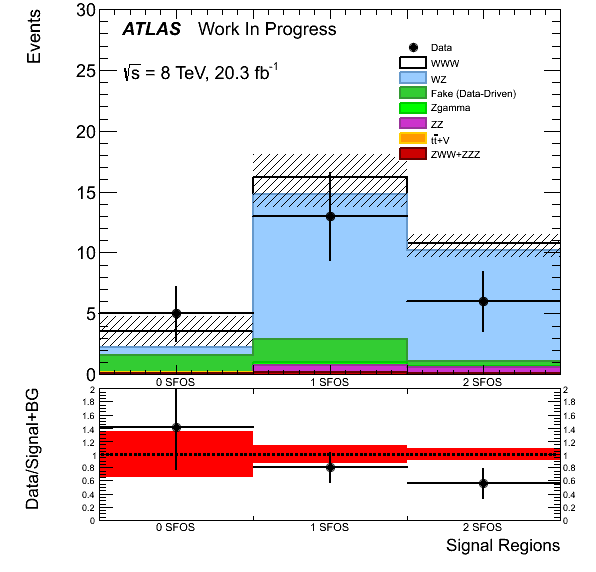
\includegraphics[width=0.5\columnwidth]{figures/SFOSSignalRegions.png}
%\caption{Yields after full selection in the 0, 1 and 2 SFOS regions.  The most important systematic uncertainties are shown, namely from the fake estimates and the uncertainties on the WZ and ZZ k-factors.}
%\label{fig:sig_yields_nsfos}
%\end{figure}
